\subsection{Solución actividad 1}
\noindent \textbf{Actividad 1}\\
En la Figura 28 se muestran 5 sistemas diferentes, de los cuales se deben identificar las variables f´ısicas,
los elementos almacenadores de flujo, de esfuerzo, disipadores y fuentes de energ´ıa, una vez identificados los
sistemas, llenar la tabla mostrada en la Figura29.\\

\begin{center}
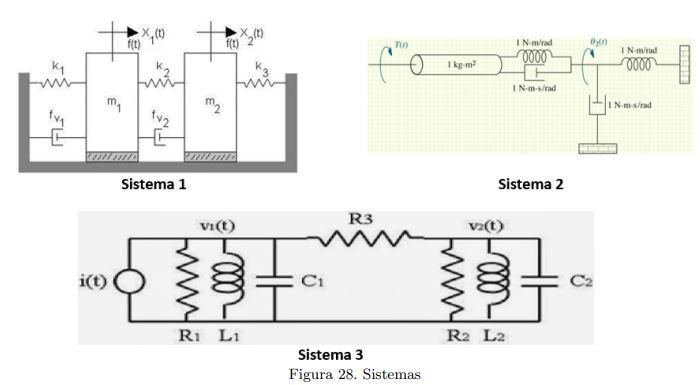
\includegraphics[scale=0.6]{img1.jpg} 
\end{center}

\begin{table}[t]
\begin{center}
\begin{tabular}{| c | c | c | c | }

\hline
Actividad & Sistema 1 & Sistema 2 & Sistema 3 \\ \hline
Tipo & mecánico translacional. & mecánico rotacional. & eléctrico. \\ \hline
& x & $\theta$ & v \\ 
Variables físicas  & v & $\omega$ & i \\ 
& a & $\alpha$ &  \\ \hline

Almacenadores de flujo & m$_{1}$ & m$_{1}$ & C$_{1}$ \\
& m$_{2}$ &  & C$_{2}$ \\ 
& $\dot{x}=\frac{p}{m}[kg]$ & $\omega=\frac{H}{I}[Nms^{2}]$ & $i=\frac{\lambda}{L}[Vs/A]$ \\
&  &  &  \\
Leyes de c. general& $a=\frac{1}{m}\frac{d}{dt}p$ & $\alpha=\frac{1}{J}\frac{d}{dt}h$ & $i_{c}=C\frac{d}{dt}VC$ \\ \hline

& k$_{1}$ & k$_{1}$ & L$_{1}$ \\ 
Almacenadores de esfuerzo & k$_{2}$ & k$_{2}$ & L$_{2}$ \\ 
& k$_{3}$ &  &  \\
& $F=Kx[N/m]$ & $\tau=K_{\omega}\omega[Nm/rad]$ & $e=\frac{q}{C}[As/V]$ \\
&  &  &  \\
Leyes de c. general& $f_{12}=Kx_{12}$ & $\tau=K_{\theta}\theta_{12}$ & $V_{L}=L\frac{d}{dt}iL$ \\ \hline

fuentes de energía & f$_{1}$(t) & $\tau$ & i \\ 
& f$_{2}$(t) &  &  \\ \hline

Elementos disipadores & fv$_{1}$ & f$\omega$ $_{1}$ & R$_{1}$ \\
& fv$_{2}$ & f$\omega$ $_{2}$ & R$_{2}$ \\
&  &  & R$_{3}$ \\ 
& $F=b\dot{x}[Ns/m]$ & $\tau=b_{\omega}\theta[Nms]$ & $e=Ri[\Omega]$ \\
&  &  &  \\
Leyes de c. general& $f_{12}=Kx_{12}$ & $\tau=K_{\theta}\theta_{12}$ & $V_{L}=L\frac{d}{dt}iL$ \\ \hline


\end{tabular}
\caption{Figura 29. Identificación de sistemas físicos.}
\end{center}
\end{table}